\chapter{Background}\label{C:back}

\section{Network packet}

\par Communication between computers is established through the means of physical connections and protcols overlaying on top of this. 
A widespread communication protocol is to break down each point of communication into discrete pieces called network packets.
These network packets contain many layers (Figure: \ref{fig:OSIModel}) of communication information.
Communication layers can be broken down into a few independent layers which hold specific purposes. 
Each layer contains information which can aid with transporting the information to the correct computer securely.
As each layer is independent, each higher layer does not affect the forthcoming layers.
High layers of the model are for purposes such as reliability of data and the data itself in the packet.
For the purposes of this project, an explanation of only the first three layers of the Open Systems Interconnection (OSI) model is concerned.

\begin{figure}[H]
    \begin{center}
        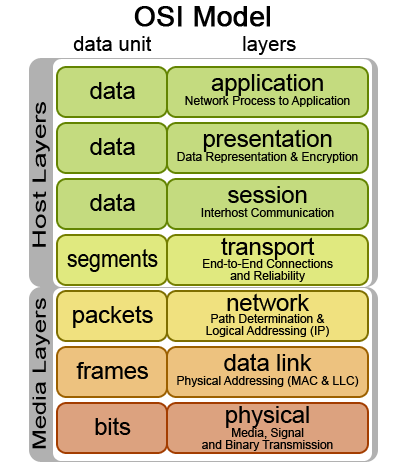
\includegraphics[width=5cm,height=5cm,keepaspectratio]{Images/OSIModel.png}
        \caption{OSI Model}
        \label{fig:OSIModel}
    \end{center}
\end{figure}

\subsection{Layer 1: Physical}

\par The physical layer is specifying the electrical and physical medium that is used to transport individual bits from one computer to another.
Two or more computers can be connected through many different physical mediums such as copper wiring and light fibers. 
Each medium has specific pros and cons, from implementation costs to throughtput capabilities.
The physical layer is responsible for transmitting and receiveing unstructured data.
Communication can be either Simplex, Half Duplex or Full Duplex.
The network topology is defined by how the physical layer is configured.
An example of a phyiscal medium is a copper medium is used to link two devices together.
This project will be investigating the latency present in a Gigabit Ethernet system, using copper based medium.

\subsection{Layer 2: Data link}

Data link layer is responsible for node-to-node data communication. 
It links from one device to another, determing the connection status of two physically connected devices.
A feature of this layer, is the ability to detect and correct errors created at the physical layer.
The IEEE Standard 802 \cite{IEEE802} details how this layer is split into two sub layers, Media Access Control (MAC), and Logical Link Control (LLC).
This project will cover networking switches which distinguish different destination devices by their unique MAC addresses.

\subsection{Layer 3: Network}

Network layer provides functionality when sending data across a network.
End-to-end communication is aided by assigning each node in the network an address, which it identifies itself with.
This allows data to be passed through intermediate nodes, which would continue to traverse until the target node has been reached.
This project will not be including this layer, or any others higher than this, as the latency measurements involved are short, single node-to-node distances.

\section{Network Latency}

\subsection{Connection Time}

\subsection{Round Trip Time}

\section{Current Timing Solutions}

Timing of network packets can currently done through very expensive and bulky devices. 
For this reason, there are many software implementations that allow high speed packet processing.
The following software implementations have some restrictions on what hardware they can run on.
The precision to measure the latency of packets is unknown and needs to be investigated.
This project is to combine the flexibility of software and hardware to create a packet latency measurement utility.

\subsection{Data Plane Development Kit (DPDK)}

Data Plane Development Kit (DPDK) is a set of C libraries to allow for rapid processing of network packets.
It utilizes a few low level Application Programming Interfaces (APIs) to minimize the overhead of using a specific architecture computer.
Reducing this overhead of the CPU reduces the amount of latecy present in the act of measuring the time between packets itself.
This is a very good software solution to what is currently on the market, but one caveat to using this technology is that only specific hardware can be used.
The Network Interface Card (NIC) on the computer has to be compatible with the software.

\subsection{PF\textunderscore RING}

PF\textunderscore RING by ntop\texttrademark is a software solution for rapid network packet processing.
It is a network socket technology which improves the speed at which packets are captured by the processor.
Faster packet processing ensures that the time stamp placed on an ingress packet is accurate as it can be.
This is a software solution which could potentially work well, but is limited by the software latency of needing to be processed by a processor.
The NIC on the computer does not have to be a specific model, meaning this is a much more flexible solution.

\section{Measurement Techniques}

\subsection{Cut-Through}

\subsection{Store-and-Forward}

\section{Field Programmable Gate Array}

\subsection{Reconfigurable Macro Cells}

\subsection{FPGA vs Microcontroller}
